\documentclass{beamer}
\usepackage[utf8]{inputenc}
\usepackage{amssymb,amsmath,amsthm,mathtools,booktabs}

\usepackage{tikz}
\usetikzlibrary{calc} 

\newcommand{\tr}{{\text{tr}}}
\newcommand{\B}[1]{\textbf{#1}}
\newcommand{\T}[1]{\texttt{#1}}

\title{The Qudit Arthurs-Kelly Measurement...\\for SIC's!}
\author{Matthew B. Weiss}
\institute{UMB: QBism Group}
\date{9/12/25}

\begin{document}

\frame{\titlepage}

\begin{frame}
\frametitle{Historical flavor}
From \emph{Bell System Technical Journal}:
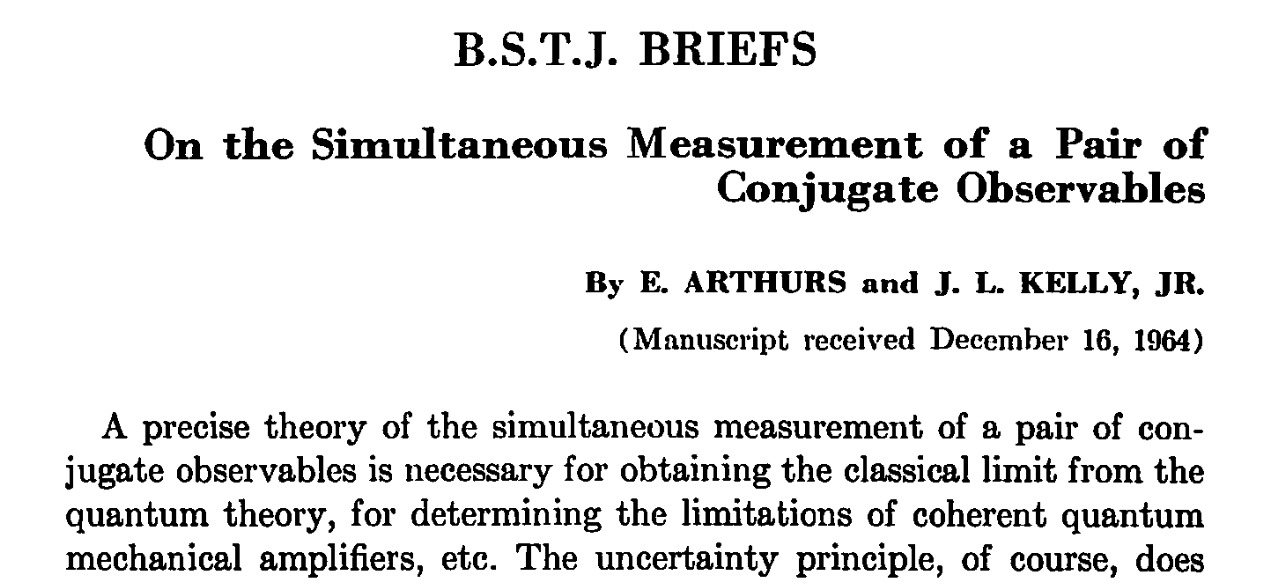
\includegraphics[scale=0.5]{img/ak_ref}	
\end{frame}

\begin{frame}
\frametitle{Arthurs-Kelly procedure}
\begin{itemize}
\item Prepare two ancillas in a special starting state.
\item Coherently shift ancilla 1 conditional on the position of the system.
\item Coherently shift ancilla 2 conditional on the momentum of the system.
\item Measure the ancillas.
\begin{itemize}
\item Realizes a ``Weyl-Heisenberg covariant POVM'' on the system.
\item E.g., coherent state measurement, or ``heterodyne'' measurement in optics.
\item Can be adapted to qudits: in particular, for a SIC measurement.
\end{itemize}
\end{itemize}
	
\end{frame}


\begin{frame}
\frametitle{Weyl-Heisenberg Group and SIC's}
Let $\mathcal{H}_d$ be a finite dimensional Hilbert space, and let $\omega = e^{2\pi i /d}$:
\begin{align}
Z|m\rangle = \omega^{m}|m\rangle && 	X|m\rangle = |m+1\rangle && D_{a,b} = X^a Z^b.
\end{align}	
Let $\Pi_{a,b}=D_{a,b}^\dagger \Pi D_{a,b}$ for fiducial $\Pi=|\phi\rangle\langle \phi|$:
\begin{align}
	\tr(\Pi_{a,b}\Pi_{a^\prime,  b^\prime})=\frac{d\delta_{aa^\prime}\delta_{bb^\prime}+1}{d+1} \Longrightarrow \text{SIC}.
\end{align}
A SIC set: regular simplex inscribed in quantum state-space!
\end{frame}

\begin{frame}
\frametitle{Qudit Arthurs-Kelly}
Let $|\cdot \rangle$ denote discrete position states and $|\cdot\rangle_p$ denote discrete momentum states.
\begin{align}
U &= \left(\sum_m I \otimes X^{-m} \otimes |m\rangle_p\langle m|_p	\right)\left(\sum_k X^{-k} \otimes I \otimes |k\rangle\langle k|\right)
\end{align}
Kraus operators: given computational basis outcomes $(x,y)$ on the ancillas, we update the system via
\begin{align}
K_{xy}=\frac{1}{\sqrt{d}}\sum_{km}\omega^{-km}\langle x+k, y+m|\gamma \rangle \ |m\rangle_p\langle k|	.
\end{align}
$|\gamma\rangle$ is the initial state of the ancillas,
\begin{align}
	\langle k,m|\gamma\rangle=\omega^{km}\langle m|F^\dagger \Pi |k\rangle,
\end{align}
where $F$ is the Fourier transform operator, and $\Pi$ is the fiducial.
\end{frame}

\begin{frame}
\frametitle{Preparing the ancillas...}
...from the fiducial:
\begin{align}
\langle k,m|\gamma\rangle&=\omega^{km}\langle m|F^\dagger \Pi |k\rangle\\
&=\langle k, m|\left(\sum_j |j\rangle\langle j|\otimes Z^j	\right)\Big(I \otimes F^\dagger\Big)\Big(|\phi^*\rangle \otimes |\phi\rangle\Big).
\end{align}
\end{frame}

\begin{frame}
\frametitle{$d=4$ SIC fiducial}
Exploit the ``monomial representation'' to write
\begin{align}
\label{fiducial}
&|\phi\rangle = \nonumber\\
&	(H \otimes I)\begin{pmatrix}1 & 0 & 0 & 0\\ 0 & e^{i\pi(-1/4)} & 0 & 0 \\ 0 & 0 & e^{i\pi (1/4)} & 0 \\ 0 & 0 & 0 & e^{i\pi (1/2)}\end{pmatrix}\frac{1}{\sqrt{5+\sqrt{5}}}\begin{pmatrix} \sqrt{2+\sqrt{5}} \\ 1 \\ 1 \\ 1 \end{pmatrix},
\end{align}	
where $H$ is the Hadamard gate.
\end{frame}

\begin{frame}
\frametitle{Qubit implementation}
	Let $\T{R}(k) = \begin{pmatrix}1 & 0 \\ 0 & e^{2\pi i/2^k} \end{pmatrix}$.
	\begin{align}
\T{Z}= \bigotimes_{j=0}^{n-1} \T{R}(j+1) && \T{X}=\T{F}^\dagger \T{Z}\T{F}.
\end{align}
Qudit Fourier transform:
\begin{center}
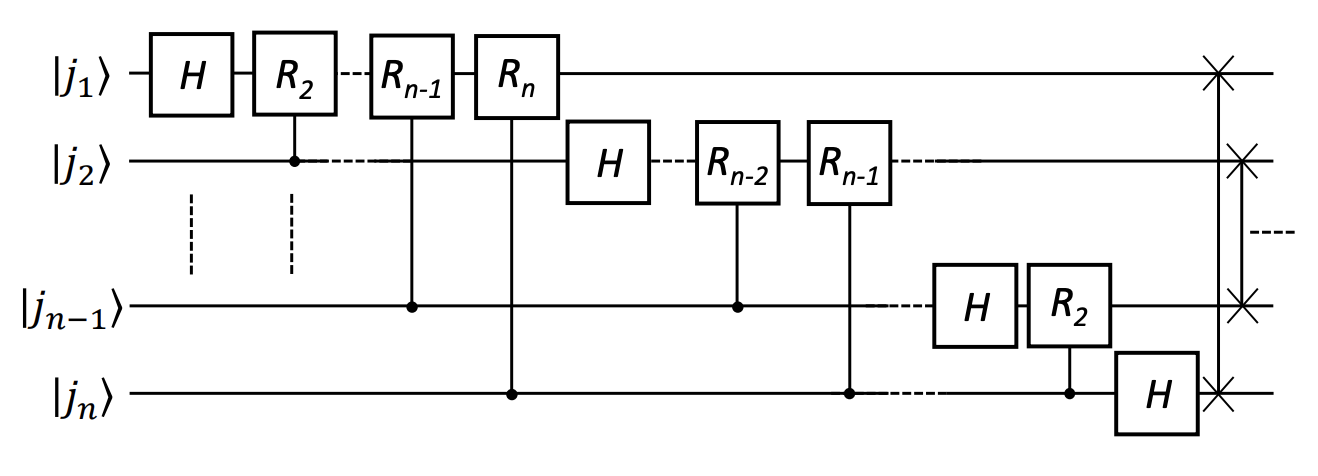
\includegraphics[scale=0.45]{img/qft.png}
\end{center}
\end{frame}

\begin{frame}
\frametitle{\T{CZ} \& \T{CX}}
\T{CZ} can be built out of a series of qudit-controlled \T{Z}'s, and \T{CX} obtained by Fourier transforming. Below: first three qubits target, second three qubits control:
\begin{center}
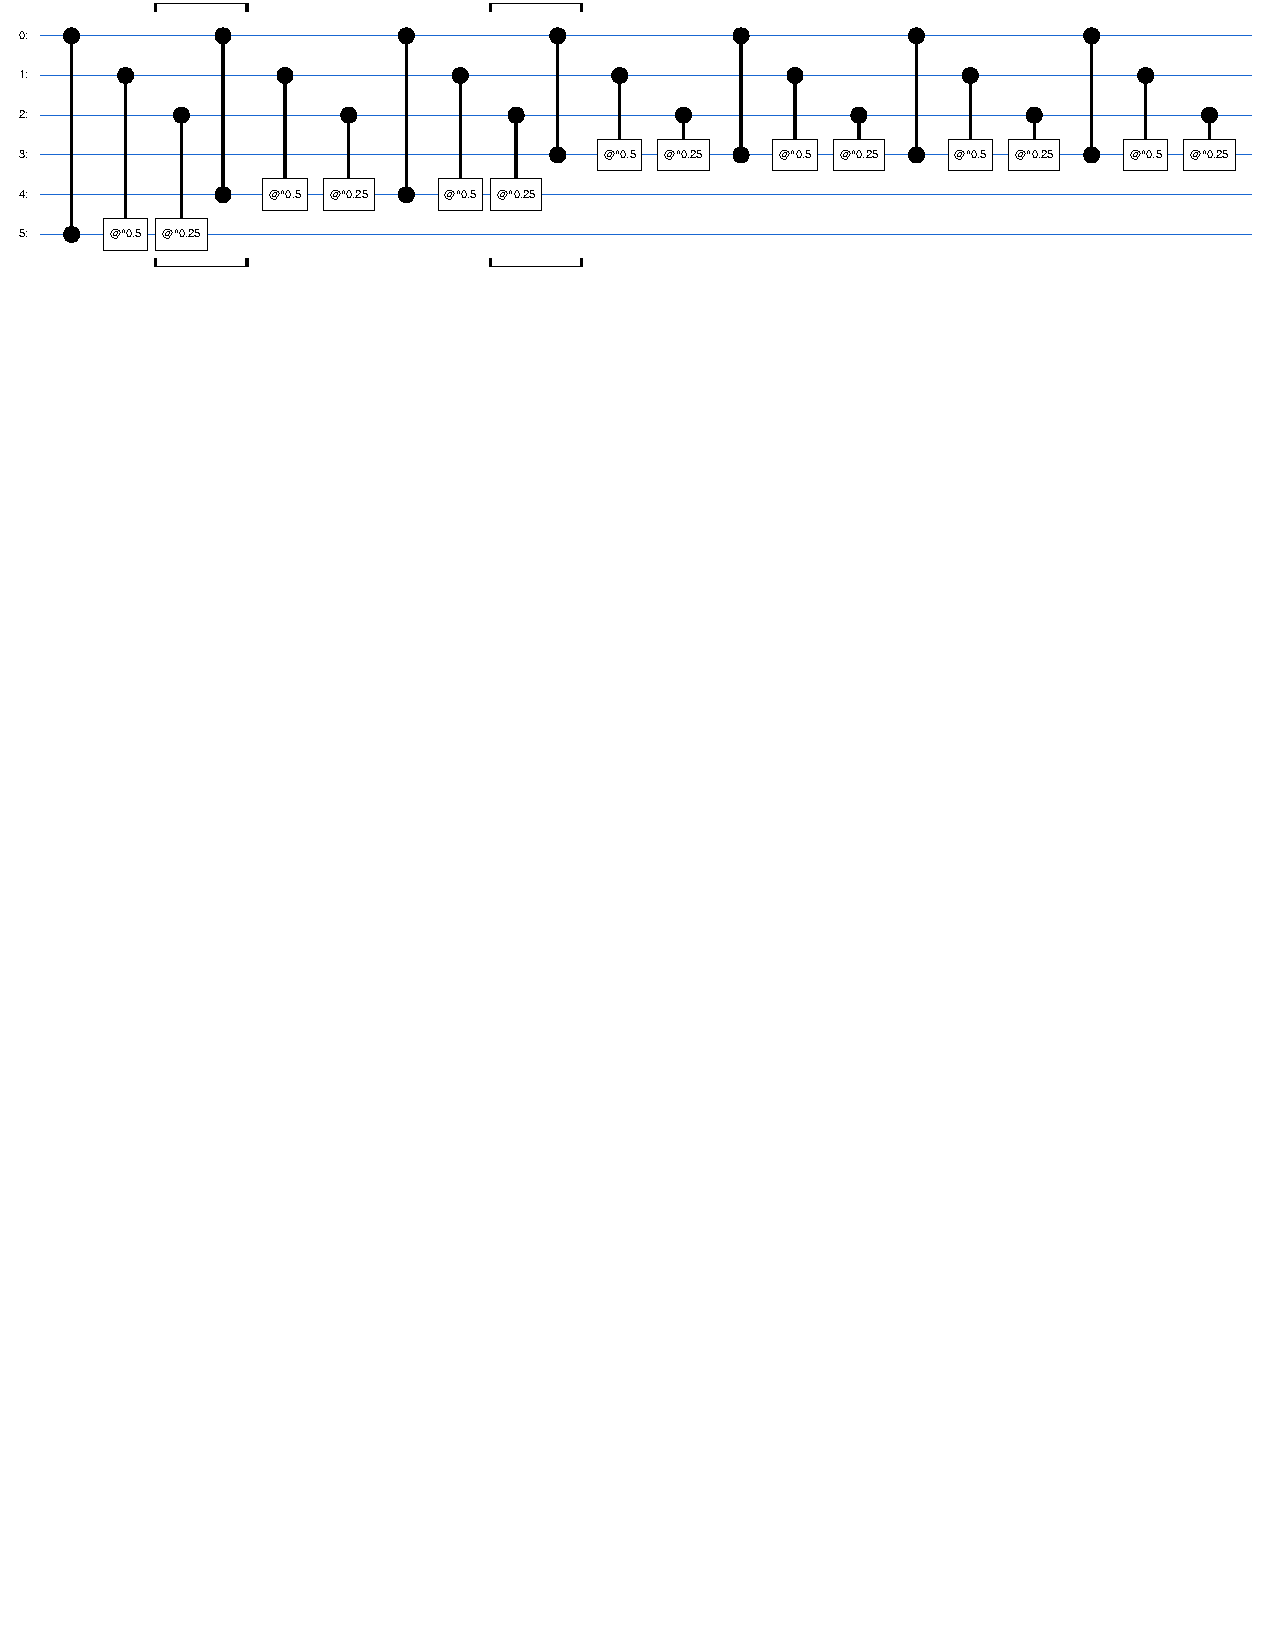
\includegraphics[scale=0.5]{img/controlled_clock.pdf}
\end{center}	
\begin{align*}
&\Big(I\otimes|0\rangle\langle0|\otimes I\otimes I + Z^4\otimes |1\rangle\langle 1| \otimes I \otimes I\Big)\\
&\Big(I\otimes I\otimes |0\rangle\langle 0| \otimes I+Z^2\otimes I\otimes |1\rangle\langle 1| \otimes I\Big)\\
&\Big(I\otimes I\otimes I\otimes |0\rangle\langle 0|+Z\otimes I\otimes I\otimes |1\rangle\langle 1|\Big)	\\
&=\sum_{m=0}^{7}Z^m \otimes |m\rangle\langle m| 
\end{align*}

\end{frame}

\begin{frame}
\frametitle{Preparing the $d=4$ fiducial}
   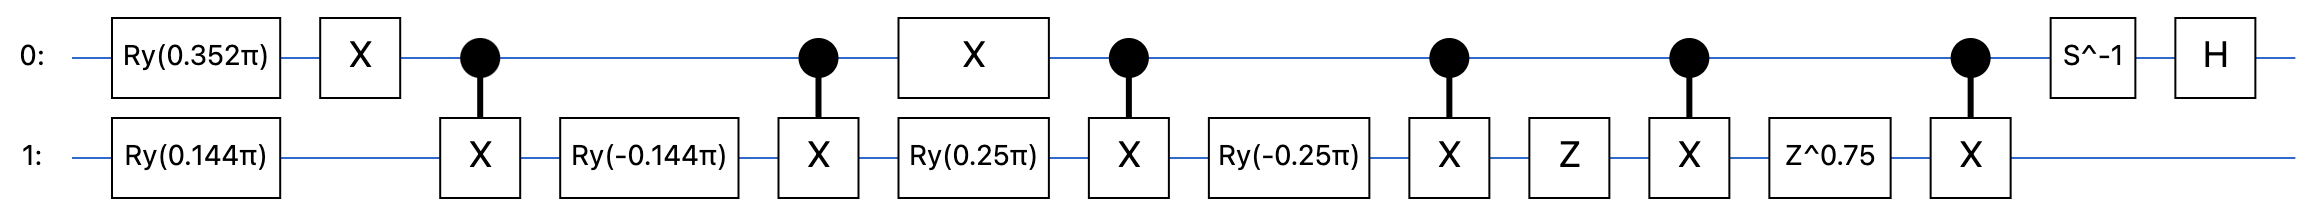
\includegraphics[scale=0.28]{img/fiducial_prep}
\end{frame}

\begin{frame}
\frametitle{Gate counts}

\begin{small}
\begin{table}[h!]
\centering
\begin{tabular}{lr lr lr}
\toprule
% Main headers spanning two columns each
\multicolumn{2}{c}{\textbf{Fiducial preparation}} & 
\multicolumn{2}{c}{\textbf{Ancilla preparation}} & 
\multicolumn{2}{c}{\textbf{Arthurs-Kelly unitary}} \\
\cmidrule(lr){1-2} \cmidrule(lr){3-4} \cmidrule(lr){5-6}
% Sub-headers
Gate type & Count & Gate type & Count & Gate type & Count \\
\midrule
% Data rows
Ry          & 5 & SwapPowGate & 1 & HPowGate    & 12 \\
PauliX      & 2 & HPowGate    & 2 & CZPowGate   & 18 \\
CXPowGate   & 6 & CZPowGate   & 7 & SwapPowGate & 6  \\
ZPowGate    & 3 &             &   &             &    \\
HPowGate    & 1 &             &   &             &    \\
\bottomrule
\end{tabular}
\label{tab:gate_counts}
\end{table}	
\end{small}
\end{frame}

\begin{frame}
\frametitle{On Willow: SIC measurement on SIC fiducial (AK)}
\begin{center}
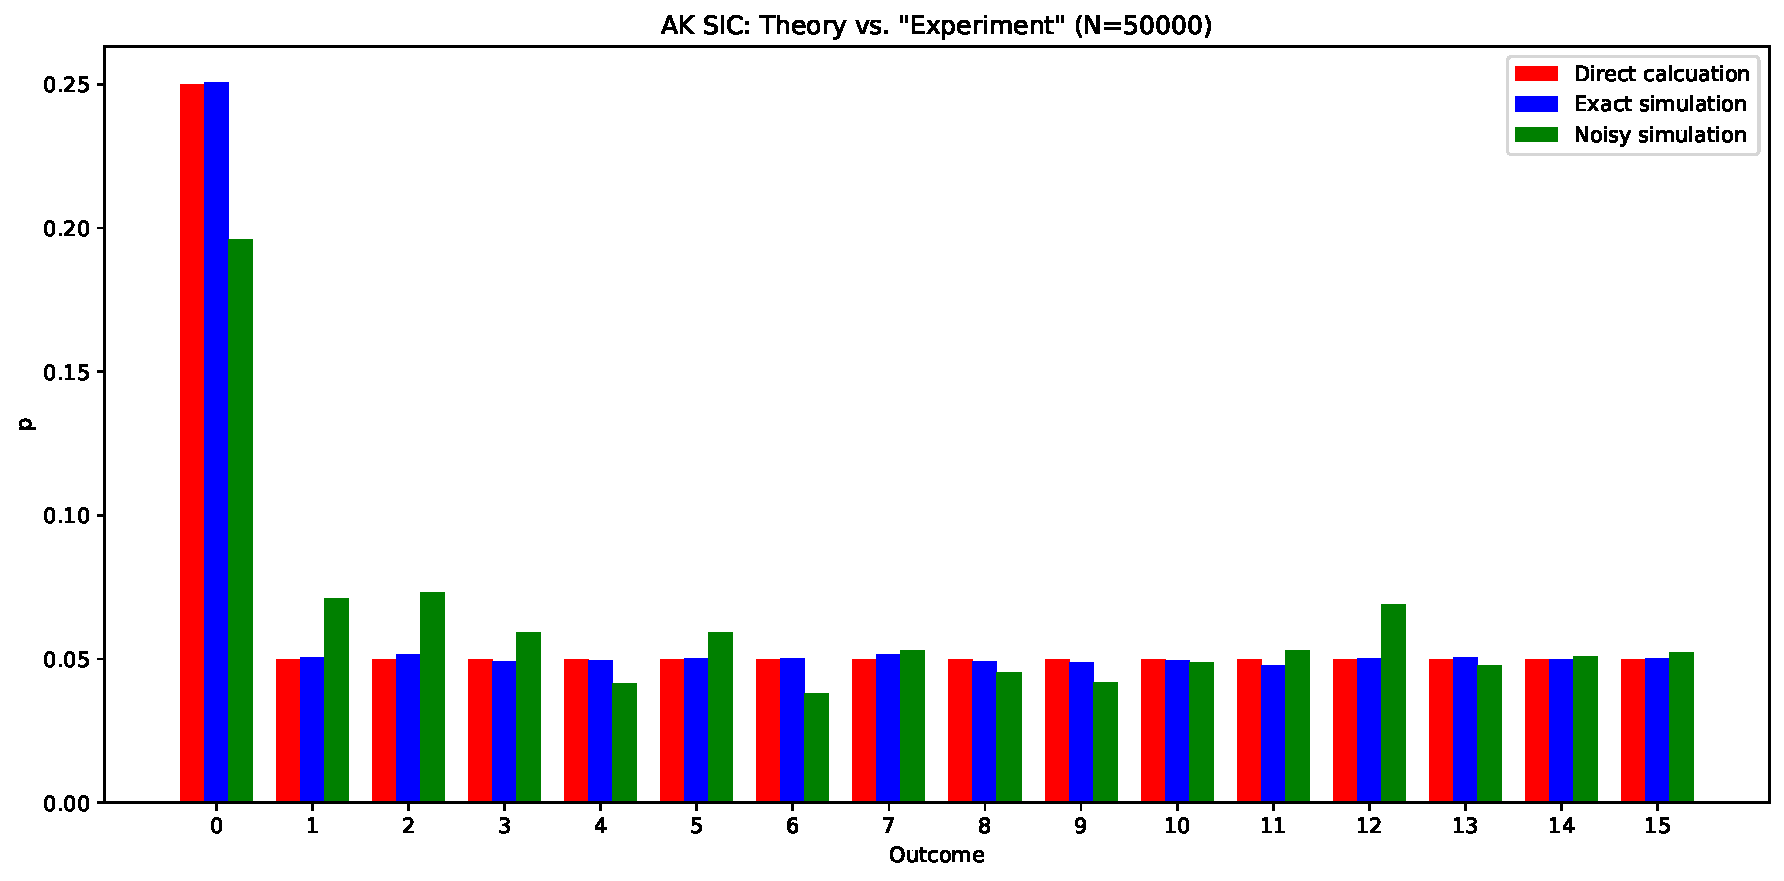
\includegraphics[scale=0.34]{img/ak_theory_vs_experiment}	
\end{center}

\begin{tiny}
\begin{table}[h!]
\centering
\begin{tabular}{lr}
\toprule
\textbf{Gate Type} & \textbf{Count} \\
\midrule
PhasedXZGate    & 67 \\
CZPowGate       & 84 \\
PhasedXPowGate  & 99 \\
ZPowGate        & 10 \\
MeasurementGate & 1 \\
\bottomrule
\end{tabular}
\label{tab:circuit_gate_counts}
\end{table}
\end{tiny}
\end{frame}

\begin{frame}
\begin{center}
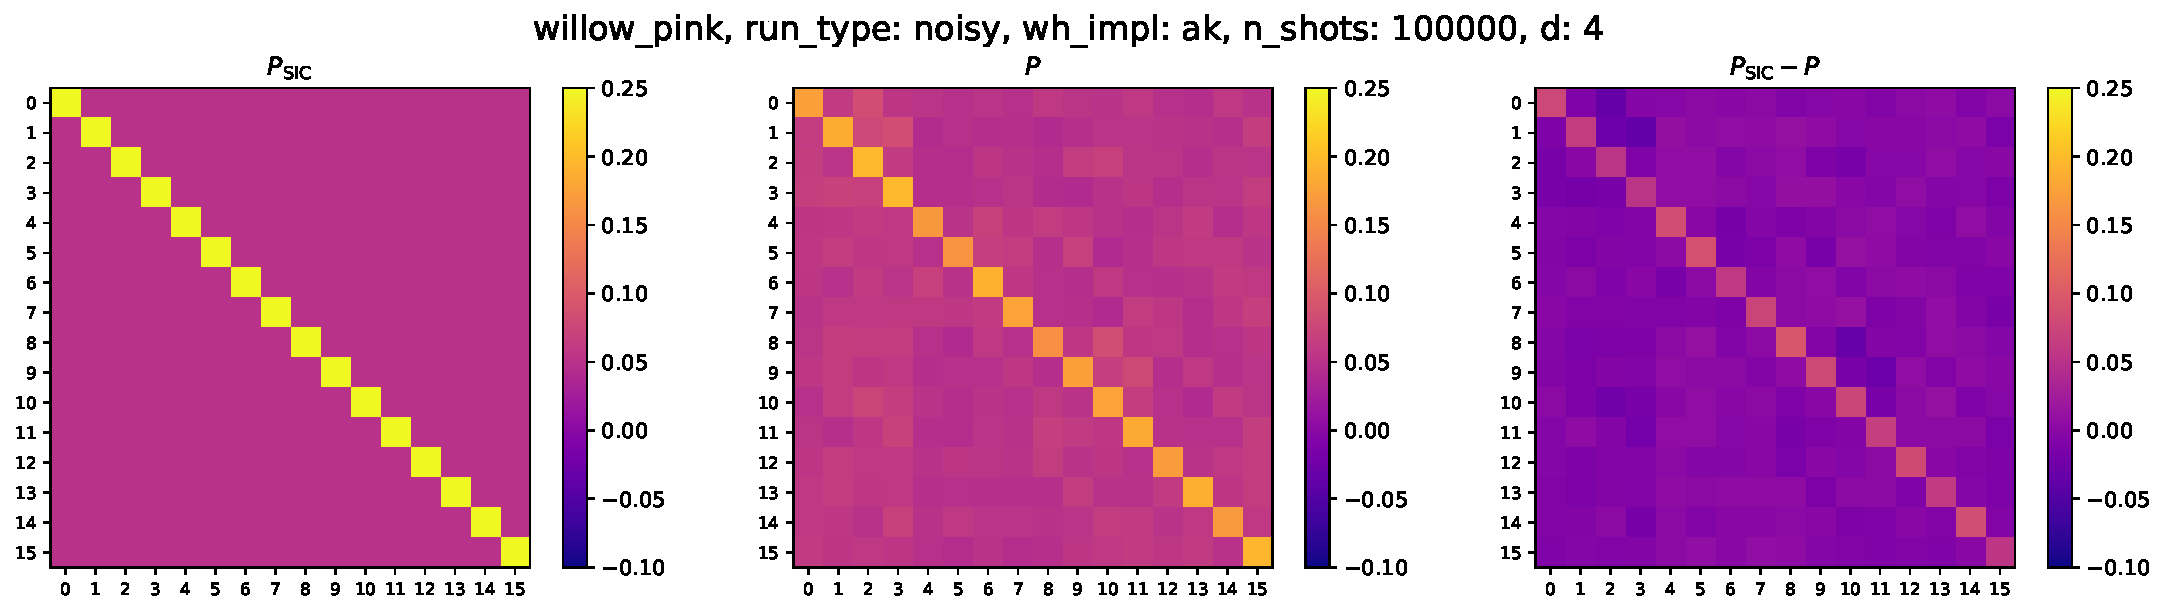
\includegraphics[scale=0.3]{img/P_noisy_ak_100000}	
$\lVert P_{\text{SIC}}-P\rVert \approx 0.3225$.
\end{center}	
\end{frame}


\begin{frame}
	\frametitle{A simplification}
Let  $|\psi\rangle$ an arbitrary state, and $|\phi\rangle$ be the fiducial.
\begin{align}
&\Big(\langle a| \otimes \langle b|\Big)(I\otimes F^\dagger)\left(\sum_j X^{-j}\otimes |j\rangle\langle j|\right)\Big(|\psi\rangle \otimes |\phi^*\rangle	\Big)\nonumber\\
&=\frac{1}{\sqrt{d}}\langle \phi |D_{a,b}^\dagger |\psi\rangle=\frac{1}{\sqrt{d}}\langle \phi_{a,b}|\psi\rangle:
\end{align}
The probabilities for a computational basis measurement are precisely the SIC probabilities. Just one ancilla!
\begin{table}[h!]
\centering
\begin{tabular}{lr}
\toprule
\textbf{Gate Type} & \textbf{Count} \\
\midrule
HPowGate    & 6 \\
CZPowGate   & 9 \\
SwapPowGate & 3 \\
\bottomrule
\end{tabular}
\label{tab:gate_counts_3}
\end{table}
\end{frame}


\begin{frame}
\frametitle{On Willow: SIC measurement on SIC fiducial (simple)}
\begin{center}
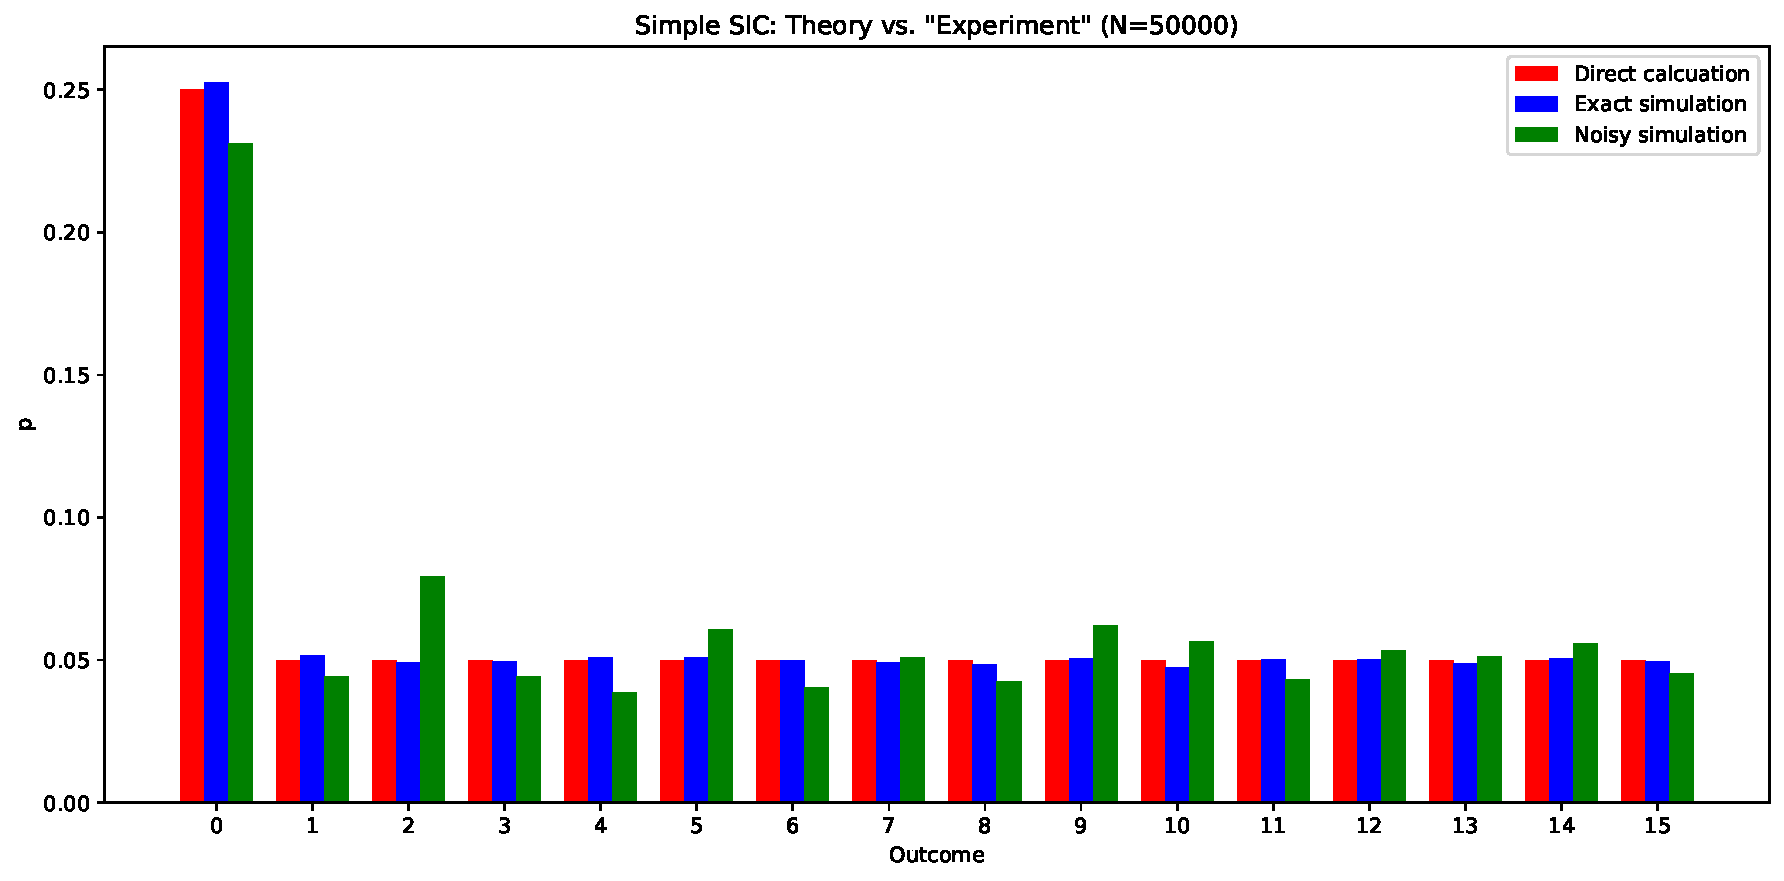
\includegraphics[scale=0.34]{img/simple_theory_vs_experiment}
\end{center}	
\begin{tiny}
\begin{table}[h!]
\centering
\begin{tabular}{lr}
\toprule
\textbf{Gate Type} & \textbf{Count} \\
\midrule
PhasedXPowGate  & 30 \\
CZPowGate       & 25 \\
PhasedXZGate    & 20 \\
MeasurementGate & 1 \\
\bottomrule
\end{tabular}
\label{tab:circuit_gate_counts_2}
\end{table}
\end{tiny}
\end{frame}

\begin{frame}
\begin{center}
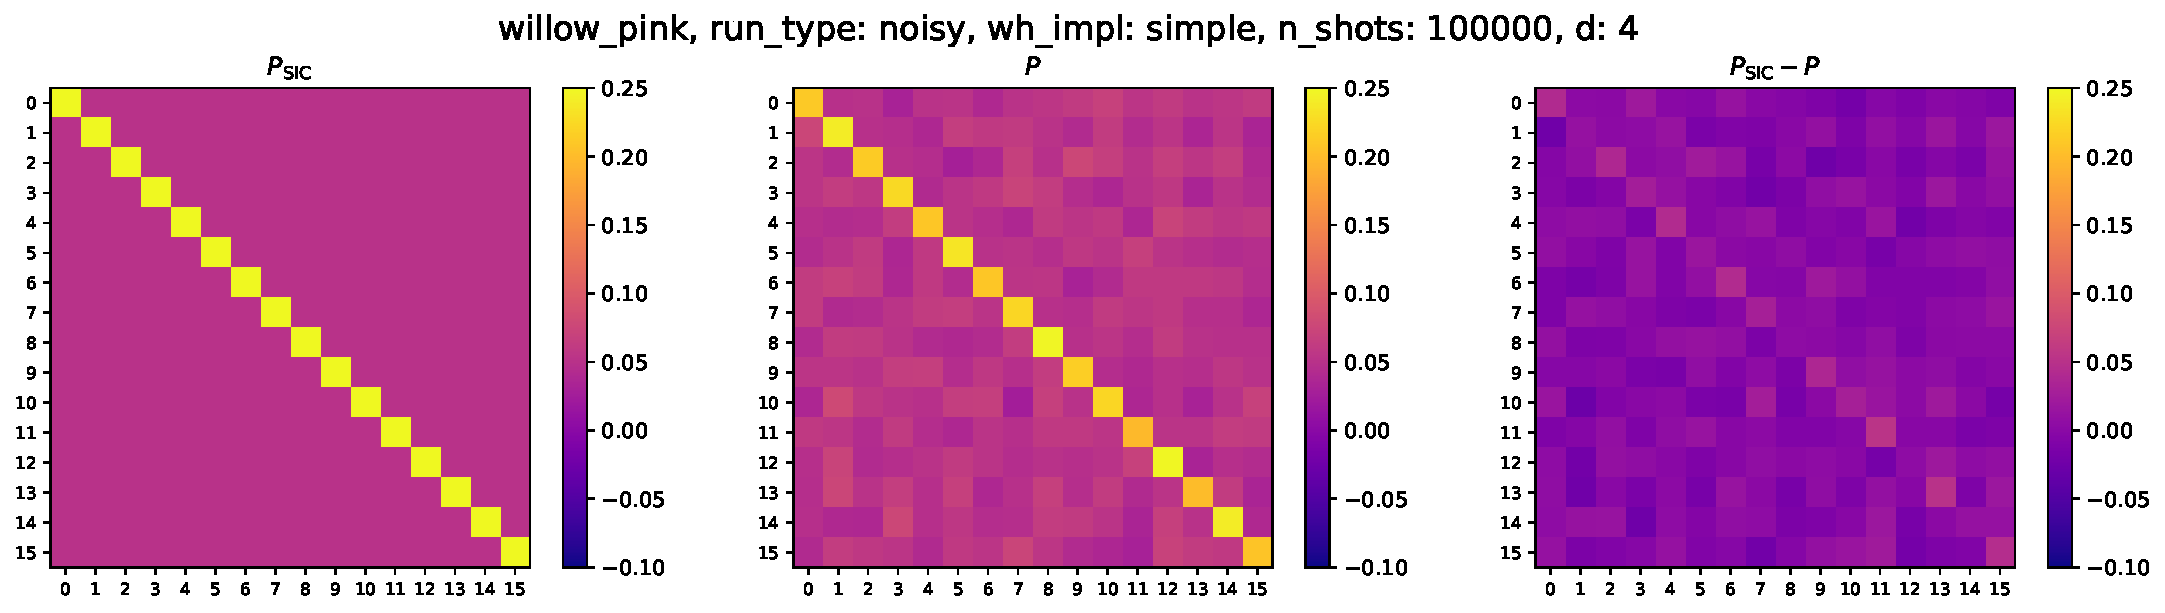
\includegraphics[scale=0.3]{img/P_noisy_simple_100000.pdf}	
 $\lVert P_{\text{SIC}}-P\rVert|=0.2126$.
\end{center}
	
\end{frame}


\begin{frame}
\frametitle{The Born Rule}
\vspace{-2em}
\begin{center}
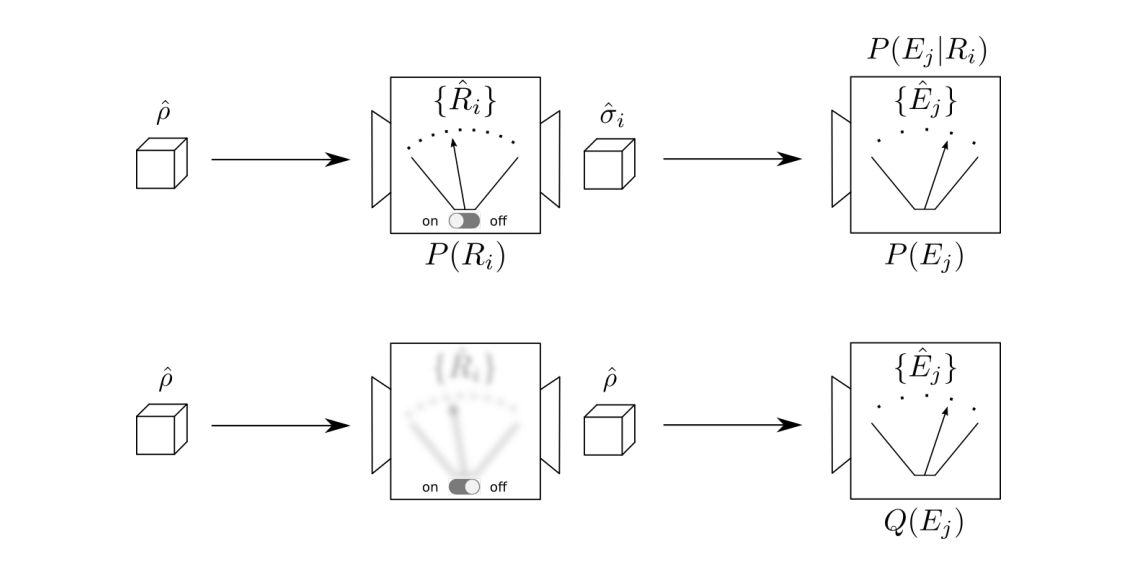
\includegraphics[scale=0.45]{img/sky_ground}	
\end{center}
\vspace{-2em}
\begin{small}
\begin{align}
P(E_j) &= \sum_i P(E_j|R_i)P(R_i)\\
Q(E_j) &= \sum_{ik} P(E_j|R_i)\Phi_{ik}P(R_k)\\
&=\sum_{i} P(E_j|R_i)\left[(d+1)P(R_i)-\frac{1}{d}\right]
\end{align}
where $\Phi = P(R|R)^{-1}$.
\end{small}
\end{frame}

\begin{frame}
\frametitle{Consistency}
Let us consider the following set of experiments:
\begin{enumerate}
\item Preparing the SIC states in turn, and then a SIC measurement. Yields matrix of probabilities $P_{ij}=f(R_i|R_j)$.
\item Prepare the computational basis states $\{\Pi_i=|i\rangle\langle i|\}$, and then performing a SIC. Yields probabilities $p_{ij} = f(R_j|\Pi_i)$.
\item Prepare the SIC states, and a computational basis measurement: $C_{ij}=f(\Pi_i|R_j)$.
\item Prepare the computational basis states, and then a computational basis measurement: $q_{ij}=f(\Pi_i|\Pi_j)$.
\end{enumerate}
	Letting $\Phi=P^{-1}$, the Born rule then demands the following consistency criterion,
\begin{align}
q = C\Phi p.	
\end{align}
\end{frame}

\begin{frame}
\frametitle{Errors}
\begin{center}
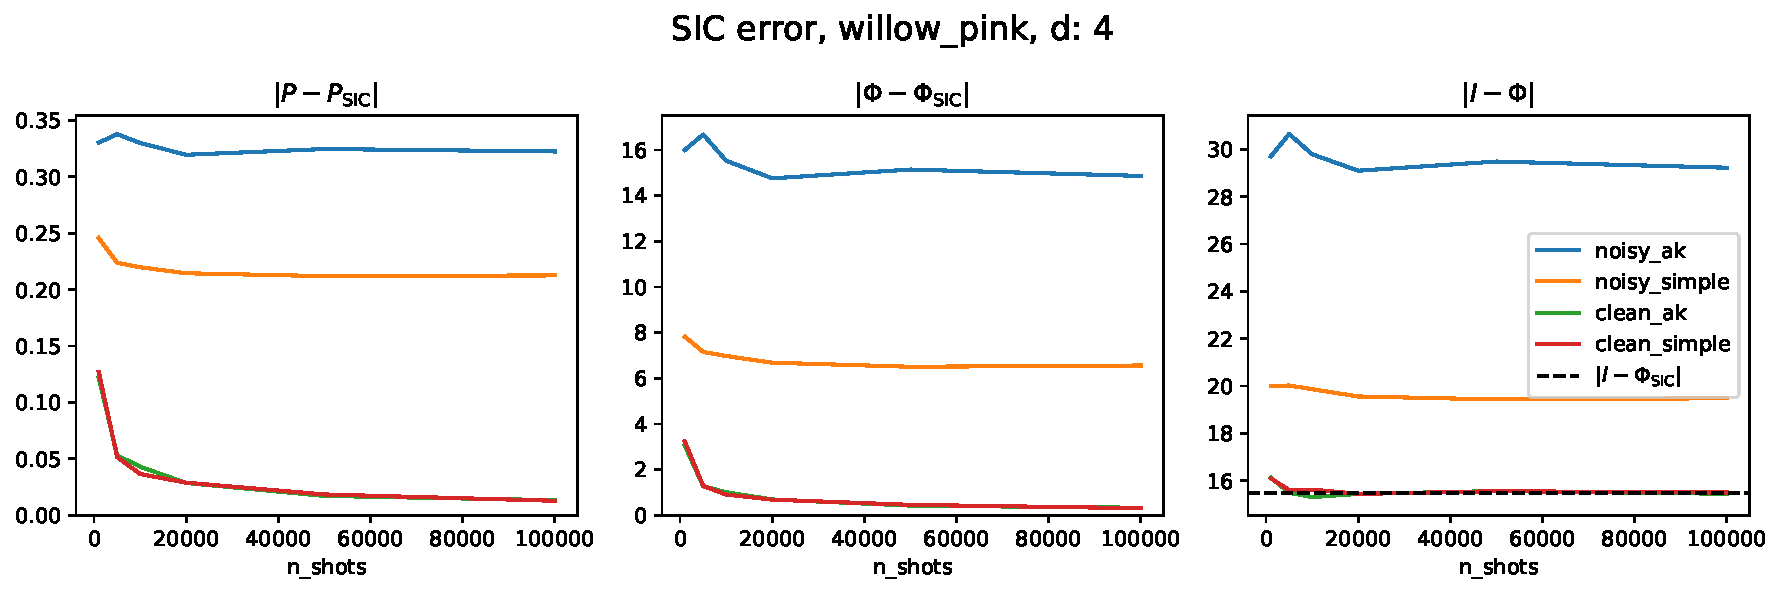
\includegraphics[scale=0.36]{img/sic_metrics}	
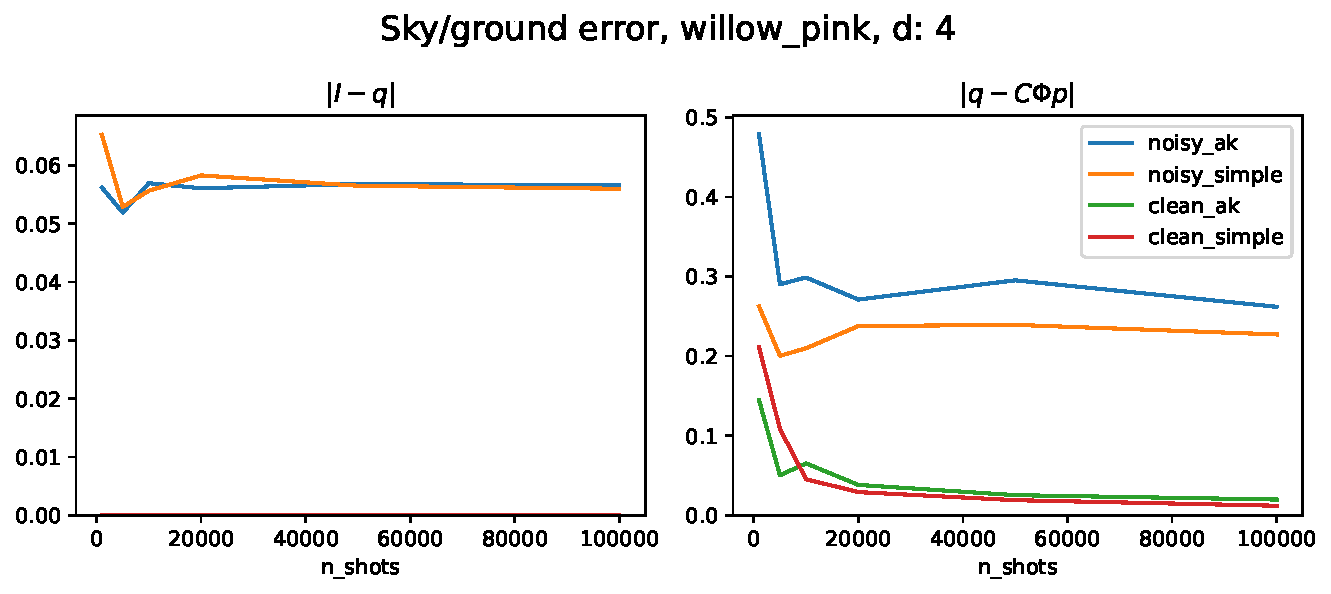
\includegraphics[scale=0.36]{img/sg_metrics}	
\end{center}	
\end{frame}

\begin{frame}
\frametitle{Errors}
\begin{center}
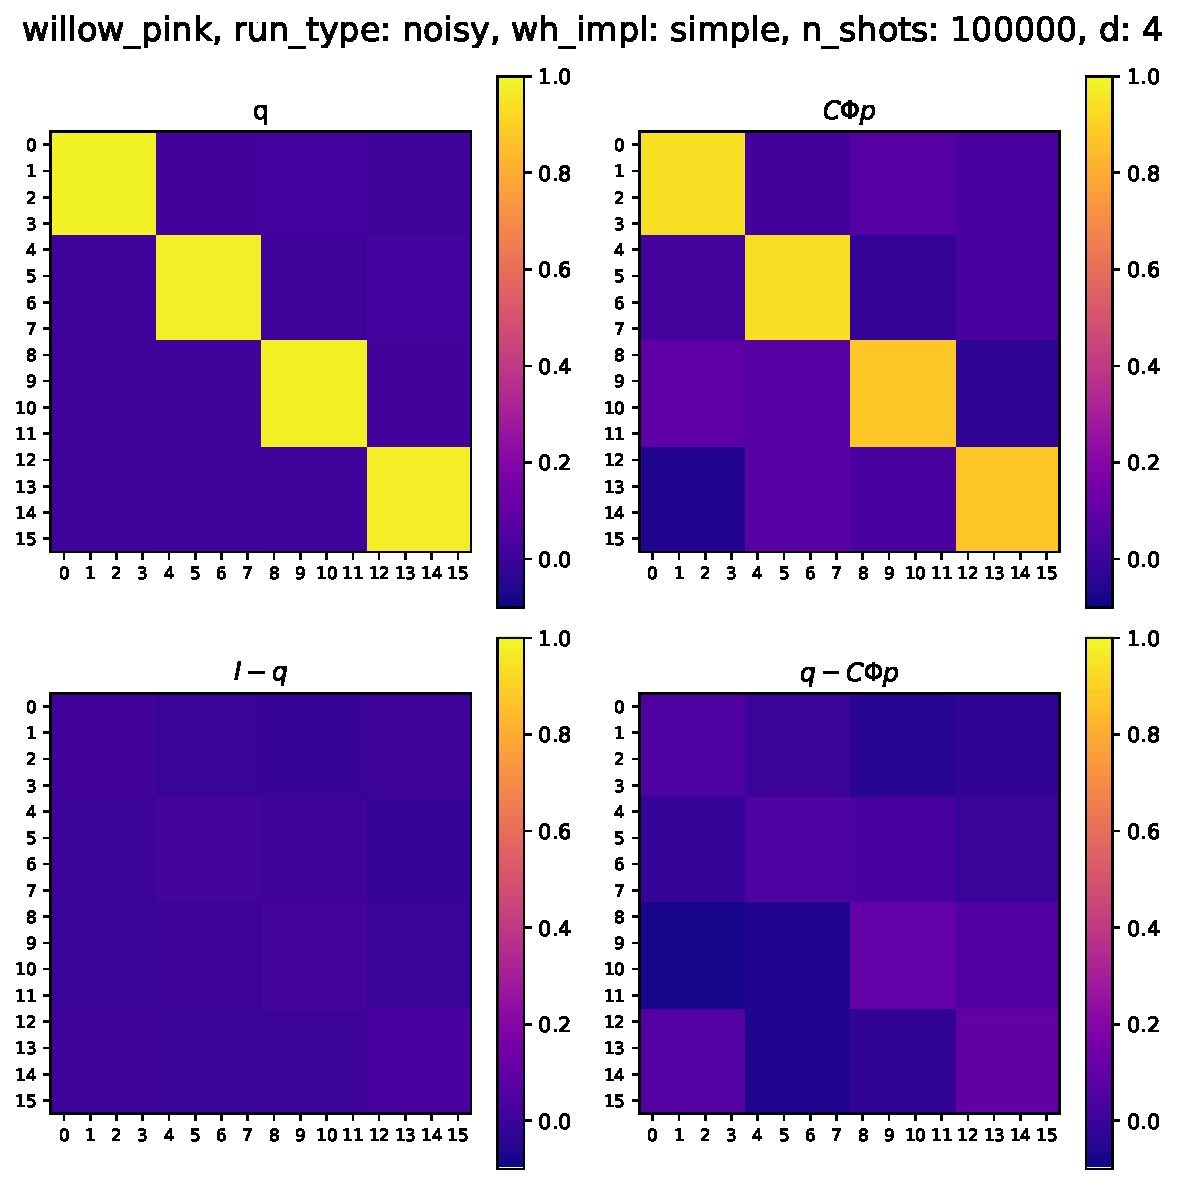
\includegraphics[scale=0.25]{img/q_noisy_simple_100000}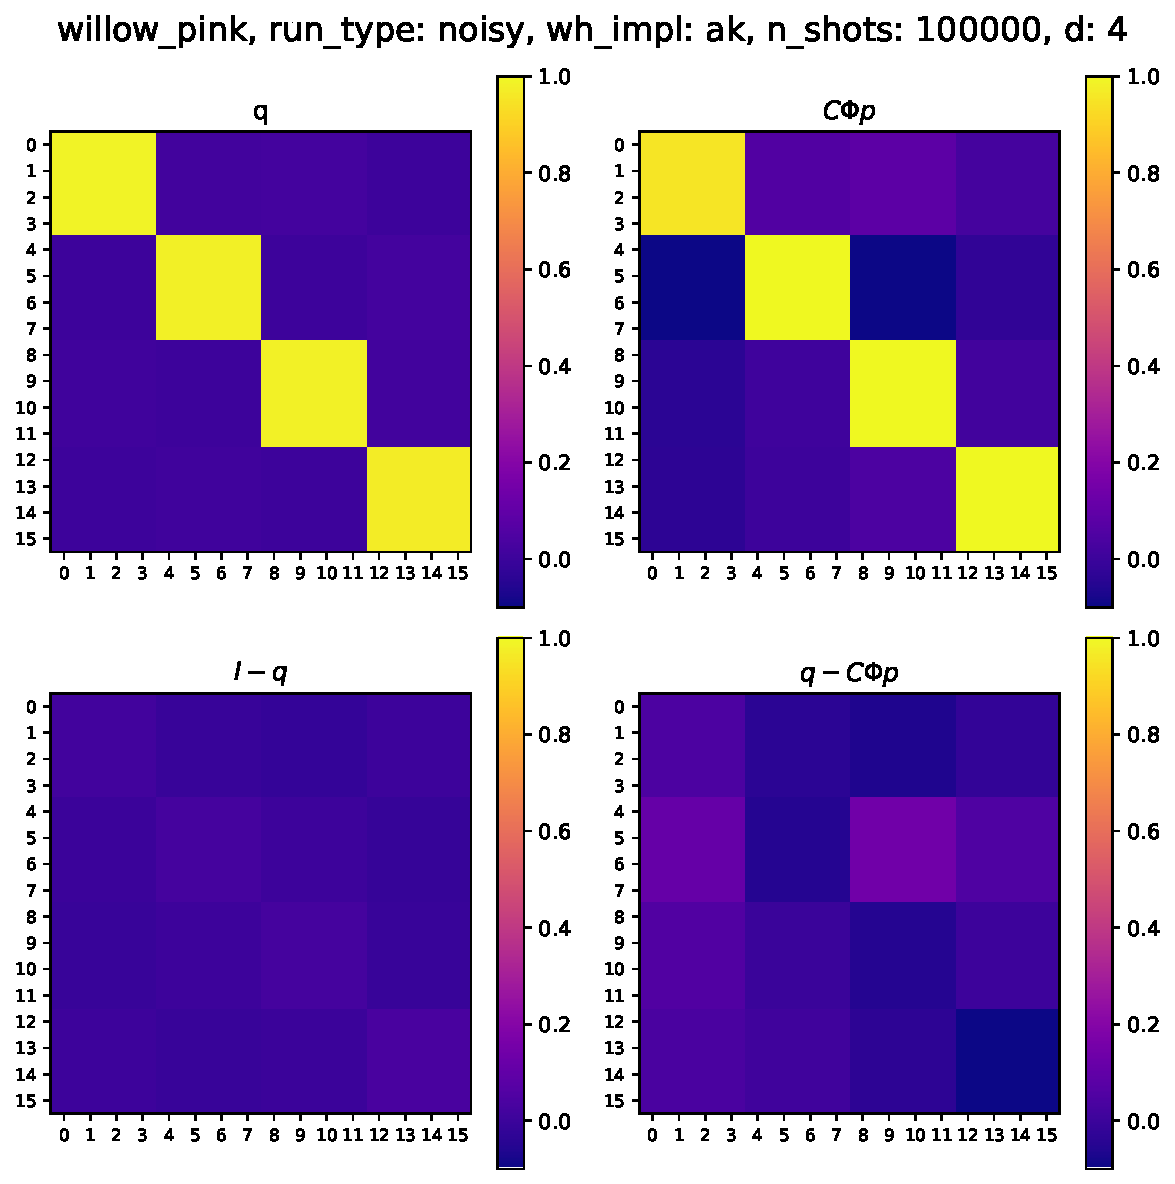
\includegraphics[scale=0.25]{img/q_noisy_ak_100000}	$\lVert I - q\rVert \approx 0.056$

$\lVert q - C \Phi p\rVert_{\text{simple}} \approx 0.2271$

$\lVert q - C \Phi p\rVert_{\text{ak}} \approx 0.2618$

\end{center}	
\end{frame}


\end{document}
